\subsection{Experimental Setup}
In our experiment, we use the Chinese part of ConceptNet which we collect by ChickenPTT~\cite{Kuo:HCOMP09} until May, 19, 2015. There are totally 713139 assertions and 223871 concepts. 

ANEW is used as our seeds. There are 1034 English words in ANEW. After our translation and expansion, these English words generate 27842 Chinese phrases. There are 3047 of them existing in ConceptNet. Among these 3047 concepts, there are 1654 positive, 1042 negative, 351 neutral according to sentiment values in ANEW. (After linear normalization, we define neutral using $\pm0.125$ as threshold.)

\subsection{Experiment 1: Propagation on the Same Topic}
This experiment aims to evaluate whether propagating on each topic separately is better than the original method which decides sentiment values from all neighbors together disregarding topics.

\subsubsection{Test Data}
From 3047 seed concepts, we sample 10\% of them to evaluate our propagation result and use the remaining 90\% as propagation seeds. To make the distributions of 10\% test data and the 90\% training data similar, we sample test data according to the proportions of positive, neutral and negative concepts. Therefore, in the test set there are totally 304 concepts where 165 of them are positive, 104 of them are negative and 35 of them are neutral.

\subsubsection{Evaluation Metrics}
We use point-wise accuracy and pair-wise accuracy to evaluate. Point-wise accuracy measures the proportion of concepts whose predicted polarities are same as their ground-truth to all test concepts. Pair-wise accuracy measures the proportion of pairs of concepts which have the same relative relation as ground-truth to all pairs.

\subsubsection{Post-Processing}
In our topic-aware results, each concept has different sentiment values on different topics. That is, each concept is associated with multiple sentiment values. To compare with original propagation, we aggregate values on different topics into one value. We compute a weighted arithmetic mean over sentiments on different topics. The weight of sentiment on topic $z$ is the proportion of valid neighbors belonging to $z$ among all valid neighbors.

\subsubsection{Results and Discussion}
The results of topic-insensitive and topic-aware propagation are discussed here. The former is the baseline, and we compare it with our topic-aware propagations with different topic numbers.

The results of point-wise and pair-wise accuracy are shown in Fig~\ref{fig:exp1_iter_pointAcc} and Fig~\ref{fig:exp1_iter_pairAcc} respectively. We can see that the performance of baseline become worse when propagating sentiments to more concepts. In contrast, topic-aware propagations with topic number $>2$ have higher and more stable point-wise accuracy and pairwise accuracy as iteration goes.

Here we investigate topic number $<=10$. Larger topic number causes topic layers of Chinese ConceptNet sparse and makes sentiment propagation fail. We found generalize contextual information into $<=10$ topics performs better.

\begin{figure}[!t]
\centering
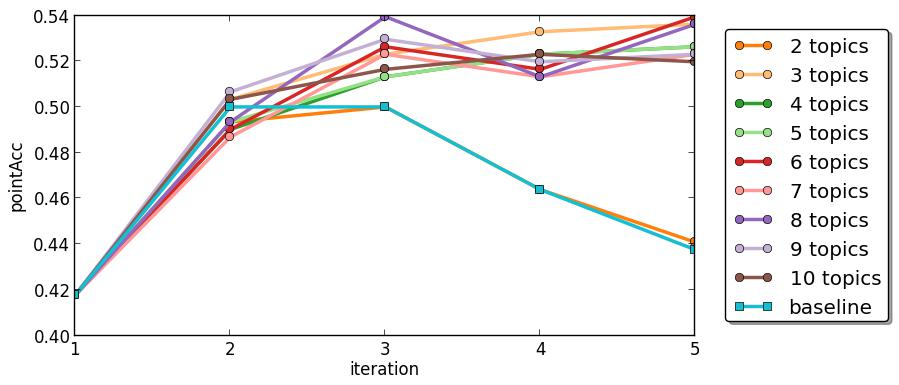
\includegraphics[width=3in]{fig/exp1_iterations/pointAcc.jpg}
\caption{Point-wise accuracy of all test concepts for the first 5 iterations.}
\label{fig:exp1_iter_pointAcc}
\end{figure}

\begin{figure}[!t]
\centering
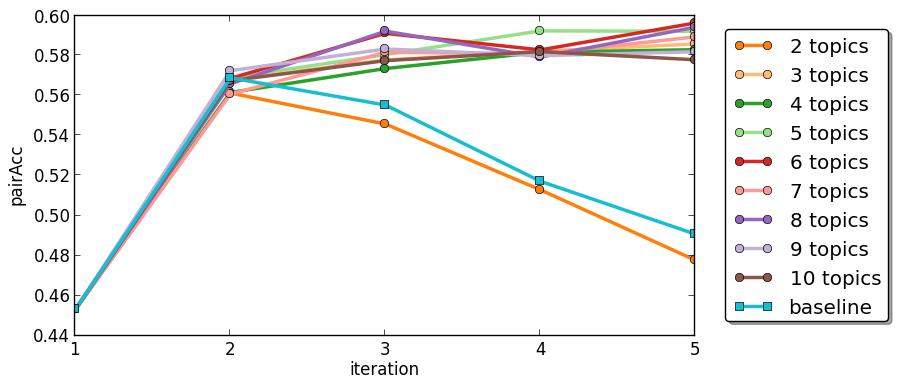
\includegraphics[width=3in]{fig/exp1_iterations/pairAcc.jpg}
\caption{Pairwise accuracy of all test concepts for the first 5 iterations.}
\label{fig:exp1_iter_pairAcc}
\end{figure}

\begin{figure}[!t]
\centering
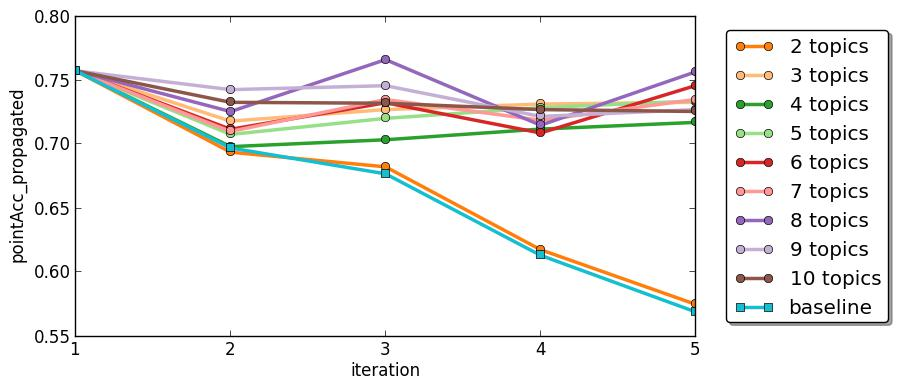
\includegraphics[width=3in]{fig/exp1_iterations/pointAcc_propagated.jpg}
\caption{Point-wise accuracy of test concepts propagated for the first 5 iterations.}
\label{fig:exp1_iter_pointAcc_known}
\end{figure}

\begin{figure}[!t]
\centering
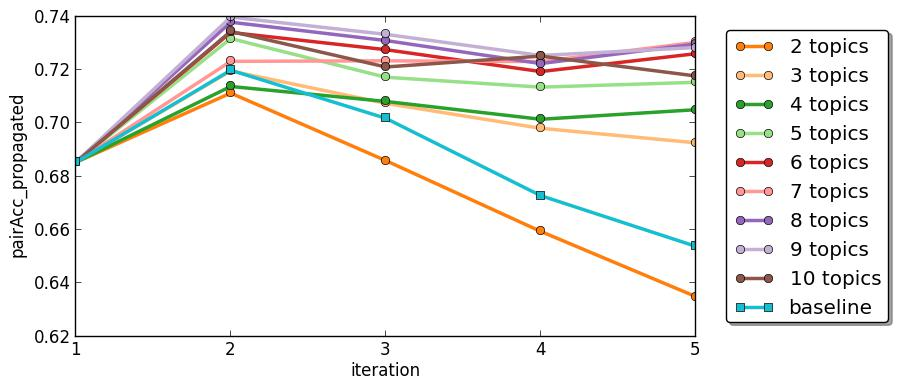
\includegraphics[width=3in]{fig/exp1_iterations/pairAcc_propagated.jpg}
\caption{Pairwise accuracy of all test concepts propagated for the first 5 iterations.}
\label{fig:exp1_iter_pairAcc_known}
\end{figure}

Some of test concepts didn't get sentiment values when propagation and are considered as neutral in our system. We exclude these concepts and investigate the performance of the remaining concepts for each iteration in Fig~\ref{fig:exp1_iter_pointAcc_known} and Fig~\ref{fig:exp1_iter_pairAcc_known}. The point-wise accuracy and pairwise accuracy reach 0.7. Except the topic number $=2$ one, topic-aware ones have higher accuracies.


%===========================
\subsection{Experiment 2: Polarity Classification for Posts of Microblog}

\subsubsection{Experimental Settings}
